\newpage
\section{INTERNAL ISSUES}




\begin{figure}[h]
     \centering
     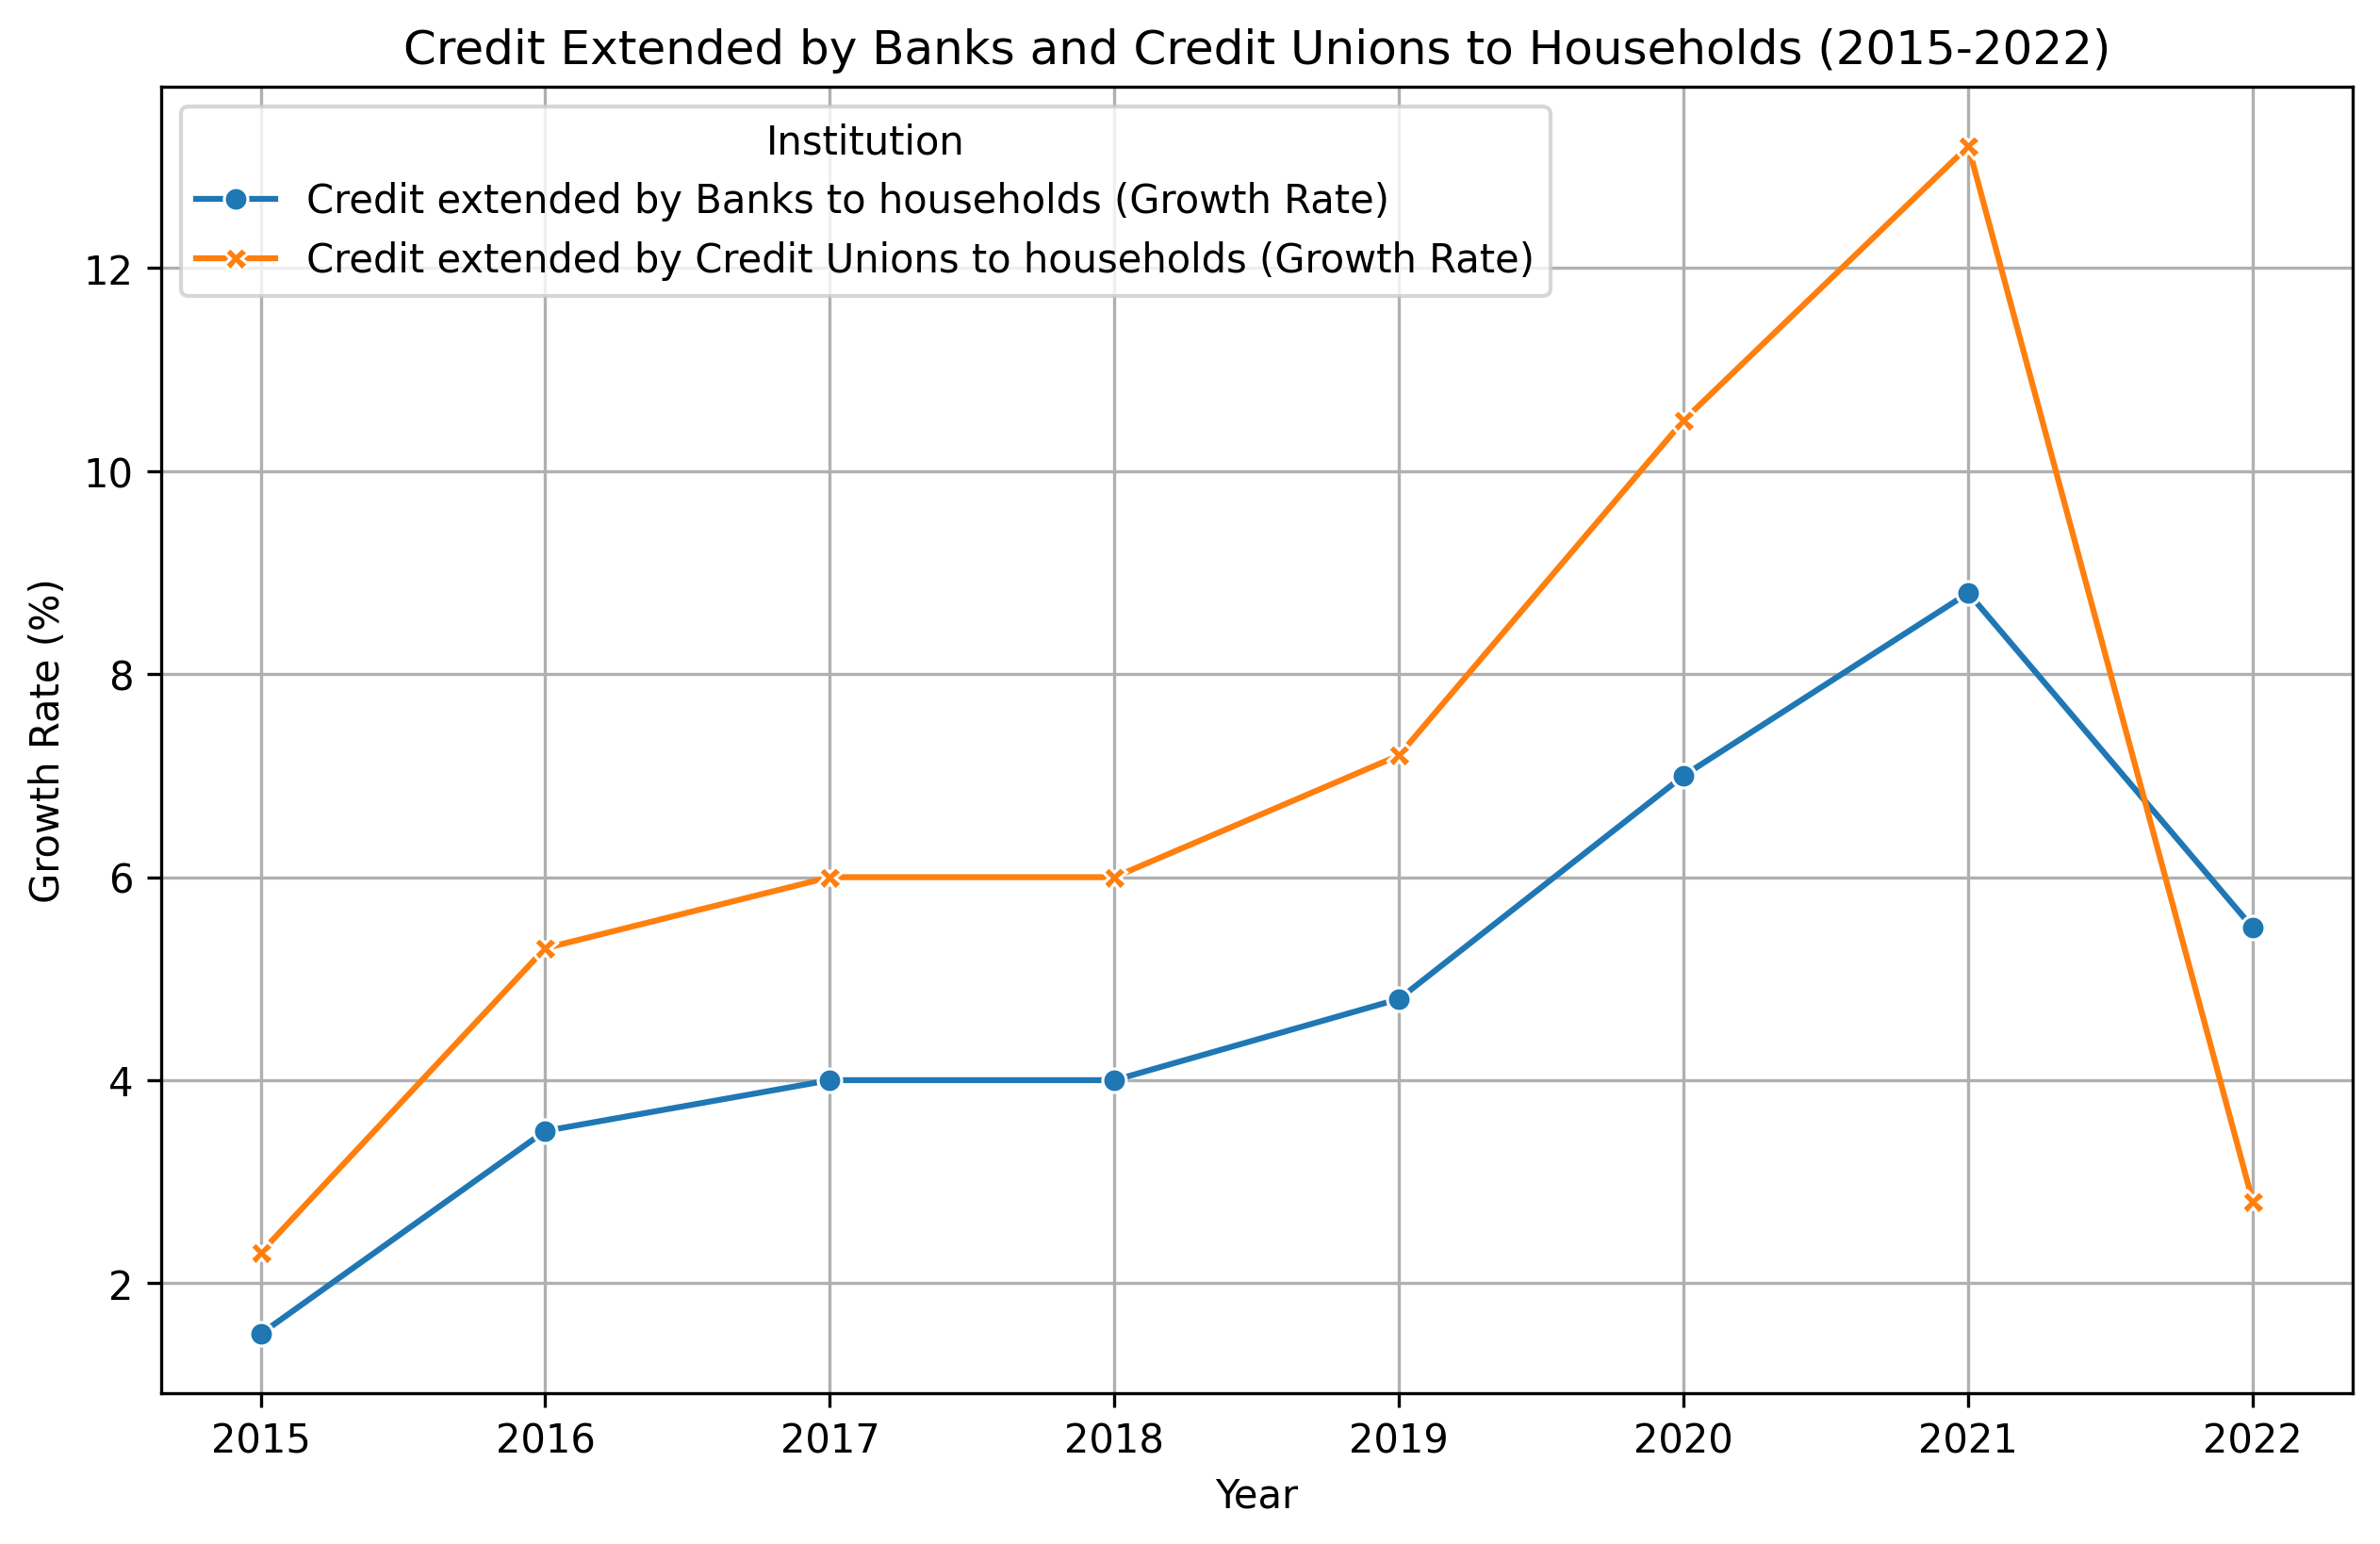
\includegraphics[width=0.8\textwidth]{graph_1.png}
     \caption{Credit Extended By Banks and Credit Unions to Households (2015 - 2022)}
     \label{fig:graph_1}
\end{figure}


\subsection*{Weak Financial Regulation and Insufficient Liquidity}

Macaronia's financial sector suffers from inadequate regulatory oversight, particularly in the near-bank financial sector. This lack of stringent regulation has allowed commercial banks and credit unions to engage in \textcolor{teal}{\textbf{high-risk lending practices}}, such as issuing subprime mortgages and accumulating excessive exposure to volatile real estate markets. The collapse of two commercial banks due to poor capitalization highlights the fragility of the financial system.

The correlation between liquidity ratios and prudential capital adequacy benchmarks (0.59) suggests that weak financial oversight has resulted in \textcolor{teal}{\textbf{undercapitalized banks}}, leaving them vulnerable to economic shocks. Furthermore, the strong correlation between credit extended by banks (0.88) and credit unions (0.81) with solvency ratios underscores how unchecked aggressive lending has weakened financial institutions, jeopardizing their solvency. The high correlation between public debt to GDP and unemployment (0.82) indicates that weak oversight has contributed to an overleveraged public sector, further destabilizing the economy.

For example, the lack of stringent capital requirements has allowed banks to operate with thin capital buffers, making them susceptible to sudden shocks. Additionally, the absence of robust stress-testing mechanisms has left regulators ill-prepared to anticipate and mitigate \textcolor{teal}{\textbf{systemic risks}}. This regulatory gap has created an environment where financial institutions prioritize short-term profits over long-term stability, leading to excessive risk-taking and financial fragility.

\newpage

\subsection*{Ratios Above Benchmarks on Paper, but Insufficient Liquidity}

\begin{figure}[h]
    \centering
    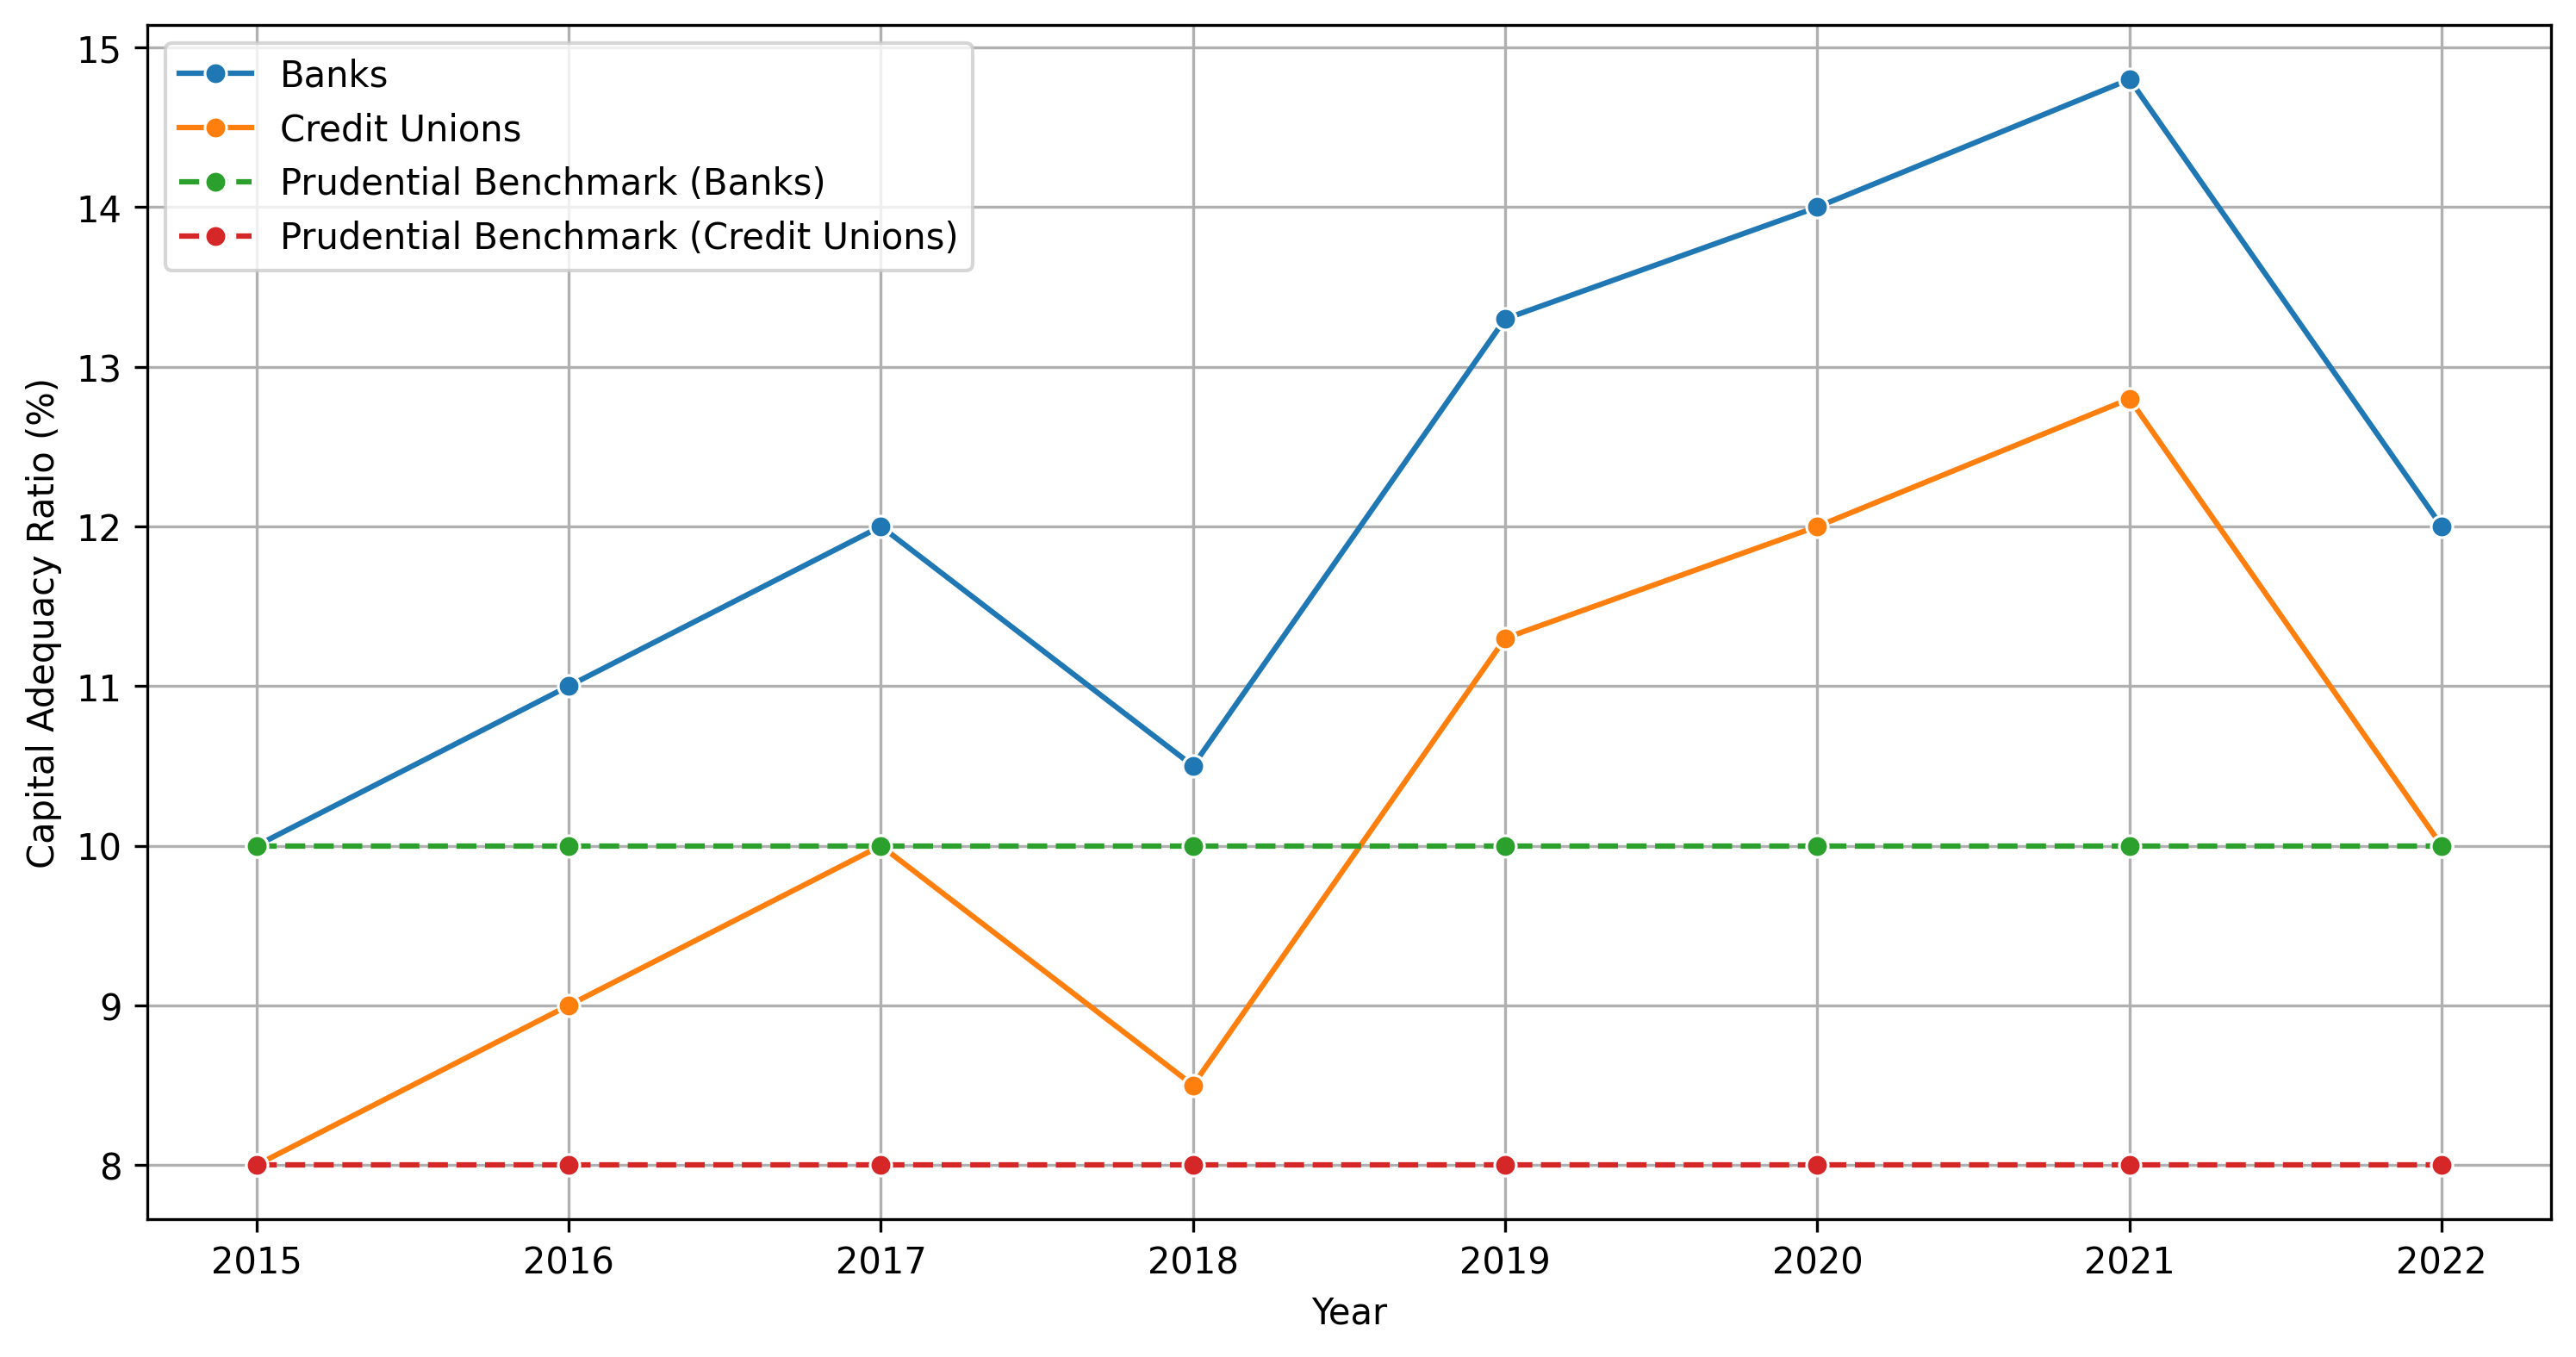
\includegraphics[width=0.8\textwidth]{Benchmarks.png}
    \caption{Credit Extended By Banks and Credit Unions to Households (2015 - 2022)}
    \label{fig:graph_1}
\end{figure}

While the \textbf{liquidity ratios} and \textbf{capital adequacy ratios} for both banks and credit unions are above the prudential benchmarks on paper, the \textbf{credit extension data} reveals a different story. On the surface, the ratios suggest that financial institutions are solvent and have sufficient liquidity to meet short-term obligations:
\begin{itemize}
    \item \textbf{Liquidity Ratios}:
        \begin{itemize}
            \item Banks: 50.0\% to 75.0\% (benchmark: 60.0\%)
            \item Credit Unions: 52.5\% to 78.8\% (benchmark: 50.0\%)
        \end{itemize}
    \item \textbf{Capital Adequacy Ratios}:
        \begin{itemize}
            \item Banks: 10.0\% to 14.8\% (benchmark: 10.0\%)
            \item Credit Unions: 8.0\% to 12.8\% (benchmark: 8.0\%)
        \end{itemize}
\end{itemize}

However, these ratios may not be sufficient to support the \textbf{scale of credit extension} in a high-risk environment like Macaronia's real estate market. Despite meeting the prudential benchmarks, the financial system is under significant strain due to \textbf{aggressive lending practices}:
\begin{itemize}
    \item \textbf{Aggressive Lending}: Banks and credit unions have extended substantial amounts of credit to households, particularly in the real estate sector. For example:
        \begin{itemize}
            \item Credit extended by banks grew from \textbf{1.5\% in 2015 to 8.8\% in 2021}.
            \item Credit extended by credit unions grew from \textbf{2.3\% in 2015 to 13.2\% in 2021}.
        \end{itemize}
    \item \textbf{High-Risk Exposure}: A large portion of this credit is tied to \textbf{high-risk mortgages} and \textbf{Real Estate Investment Trusts (REITs)}, which are highly volatile and sensitive to economic shocks.
\end{itemize}

\subsection*{Insufficient Liquidity to Support Credit Extension}

While the liquidity ratios are above the prudential benchmarks, they fall short of \textbf{international standards} required to support the level of credit extension in a high-risk environment:
\begin{itemize}
    \item According to the \textbf{Basel III framework}, banks should maintain a \textbf{Liquidity Coverage Ratio (LCR)} of at least \textbf{100\%}. This means banks must hold enough high-quality liquid assets to cover their net cash outflows for 30 days.
    \item In Macaronia's case, the liquidity ratios (50.0\% to 75.0\% for banks and 52.5\% to 78.8\% for credit unions) are \textbf{below the recommended 100\% threshold}, indicating that the financial system may not have sufficient liquidity to withstand a sudden surge in withdrawals or a sharp decline in asset values.
\end{itemize}

\subsection*{Weak Financial Regulation}

The fact that financial institutions are meeting the prudential benchmarks but still engaging in \textbf{high-risk lending} and facing \textbf{liquidity shortages} highlights the \textbf{weakness of the regulatory framework}:
\begin{itemize}
    \item \textbf{Lack of Enforcement}: Regulators may not be enforcing the benchmarks effectively, allowing banks and credit unions to operate with thin liquidity buffers.
    \item \textbf{Inadequate Stress Testing}: The absence of robust stress-testing mechanisms means that the institutions may not be prepared for severe economic shocks, such as a collapse in the real estate market.
    \item \textbf{Moral Hazard}: The presence of deposit insurance may have encouraged banks to take excessive risks, knowing that deposits are insured.
\end{itemize}

\subsection*{References to International Standards}

\begin{itemize}
    \item \textbf{Basel III Liquidity Coverage Ratio (LCR)}:
        \begin{itemize}
            \item The Basel III framework requires banks to maintain a \textbf{Liquidity Coverage Ratio (LCR)} of at least \textbf{100\%}. This means banks must hold enough high-quality liquid assets to cover their net cash outflows for 30 days.
            \item Source: \href{https://www.bis.org/bcbs/basel3.htm}{Bank for International Settlements (BIS)}
        \end{itemize}
    \item \textbf{Liquidity Ratios in High-Risk Environments}:
        \begin{itemize}
            \item In economies with high credit growth and exposure to volatile sectors, liquidity ratios should be \textbf{significantly higher} than the minimum benchmarks to account for increased risk.
            \item Source: \href{https://www.imf.org/en/Publications/WP/Issues/2016/12/31/Liquidity-Risk-and-Credit-in-the-Transmission-of-Monetary-Policy-24322}{International Monetary Fund (IMF)}
        \end{itemize}
\end{itemize}

\newpage

\subsection*{Overreliance on the Real Estate Sector}

Macaronia’s economic growth has been heavily dependent on its booming real estate market. Commercial banks and credit unions have significantly exposed themselves to Real Estate Investment Trusts (REITs), with 15\% and 25\% of their total assets tied to these instruments, respectively. However, REITs are highly volatile, particularly during economic shocks, and rely heavily on debt to finance property acquisitions and developments. They also have limited economic growth potential, tax implications, and sensitivity to interest rate fluctuations. As REIT values decline sharply, the balance sheets of financial institutions deteriorate. This erosion of equity can lead to \textcolor{teal}{\textbf{insolvency}}, limiting the institutions’ ability to lend and slowing economic activity.

The high correlations between credit extended by banks to households (0.88) and credit unions (0.81) with solvency ratios demonstrate that real estate-driven lending has been a primary factor in the financial health of banks and credit unions. The correlation between economic growth and credit union lending (0.77) underscores how the real estate boom has fueled Macaronia’s GDP expansion. However, the liquidity ratios of banks (0.61) and credit unions (0.75) alongside inflation reveal that inflationary pressures have emerged alongside credit expansion, further straining the economy. 

With REIT values declining sharply, highly leveraged banks and credit unions now face significant balance sheet deterioration, threatening their stability.

\subsection*{Aggressive Lending Practices and Economic Instability}

Aggressive lending practices have been a hallmark of Macaronia’s financial sector, driven by the real estate boom. However, this credit-fueled expansion has proven unsustainable, contributing to inflationary pressures and weakening bank balance sheets. The correlation between bank and credit union lending with economic growth (0.77) indicates that economic growth has been heavily reliant on unsustainable credit expansion. Excessive credit growth has also contributed to rising inflation, as evidenced by the correlation between liquidity ratios and inflation (0.61), further destabilizing the economy. Moreover, the strong correlation between banks’ lending and capital adequacy (0.88) shows that aggressive lending practices have directly weakened bank balance sheets, increasing systemic risk.

For example, banks have extended loans to borrowers with poor creditworthiness, often without adequate collateral. This has increased the risk of defaults, particularly in a deteriorating economic environment. Additionally, the lack of diversification in loan portfolios has left banks overly exposed to the real estate sector, amplifying the impact of sector-specific shocks.

\subsection{Currency Instability}

Macaronia’s currency has experienced significant depreciation, driven by a combination of fiscal deficits, liquidity shortages, and inflationary pressures. This instability has further exacerbated the economic crisis. The negative correlation between the exchange rate and inflation (-0.85) indicates that currency depreciation is fueling inflation, likely due to higher import costs. Persistent fiscal deficits are also driving currency instability, as shown by the correlation between fiscal deficit and exchange rate (-0.37), undermining investor confidence. Additionally, liquidity shortages are worsening currency volatility, as evidenced by the correlation between liquidity ratios and exchange rate (-0.28), creating a vicious cycle of economic instability.
For instance, the depreciation of the currency has led to a surge in the cost of imported goods, further straining household budgets and reducing consumer spending. This has had a knock-on effect on businesses, particularly those reliant on imported inputs, leading to reduced production and layoffs.haken depositor trust.

\subsection{Depositor Confidence Erosion}


The erosion of depositor confidence is a critical issue, as it threatens to trigger bank runs and further destabilize the financial system.
Declining solvency ratios and public debt concerns have shaken depositor trust. The high correlation between liquidity ratios and solvency ratios (0.94) 
suggests that depositors are withdrawing funds due to declining solvency, exacerbating liquidity issues. Depositor confidence is further undermined by concerns 
over high public debt levels, as indicated by the correlation between public debt to GDP and exchange rate (-0.68). Financial distress, reflected in the stock market decline, 
is eroding overall economic stability, as depositors and investors lose faith in the financial system.
For example, the recent collapse of two major banks has led to widespread panic among depositors, resulting in a surge in withdrawals. 
This has forced banks to liquidate assets at distressed prices, further weakening their financial position and creating a downward spiral.
